% \begin{table}[t]
% \resizebox{\columnwidth}{!}{%
% \begin{tabular}{c|ccc}
% \toprule
%     & Train & Test & Total\\
% \midrule
% CUB-200-2011 & $8232$ & $3556$ & $11788$  \\
% \midrule
% House& $217$ & $93$ & $310$\\
% \midrule
% Zoo& $196$ & $84$ & $280$\\
% \bottomrule
% \end{tabular}%
% }
% \caption{The number of images in the train and test split of each domain.}
% \label{tab:img_stats}
% \end{table}

% \begin{table}[t]
% \resizebox{\columnwidth}{!}{%
% \begin{tabular}{c|ccc}
% \toprule
%     & Train & Test & Total\\
% \midrule
% CUB & $307.8$ & $57.2$ & $365$  \\
% \midrule
% House& $34$ & $6$ & $40$\\
% \midrule
% Zoo& $28$ & $6$ & $34$\\
% \bottomrule
% \end{tabular}%
% }
% \caption{The number of concepts in the train and test split of each domain. The number of the CUB dataset comes from the average of five different splittings.}
% \label{tab:concept_stats}
% \end{table}

\begin{figure*}[h]
  \centering
\begin{subfigure}{0.28\textwidth}
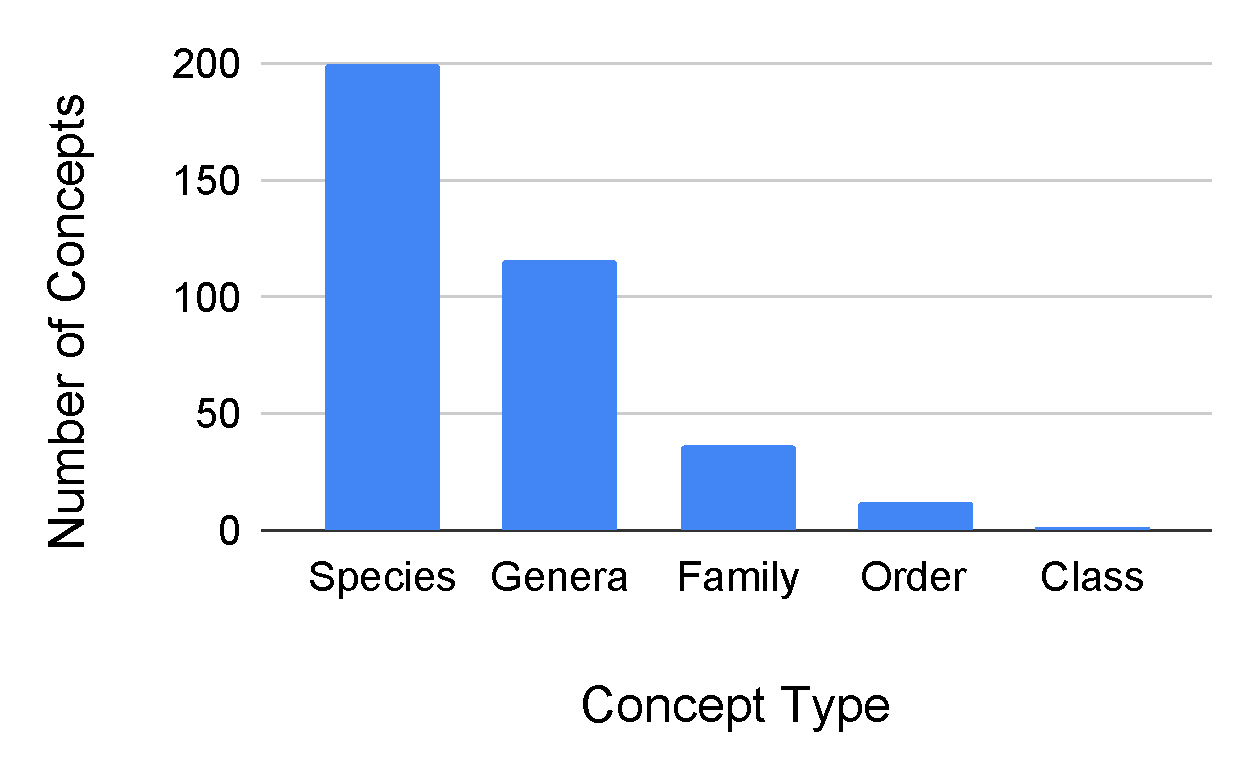
\includegraphics[width=\textwidth]{figures/chart_CUB.pdf}
  \subcaption{CUB-200-2011}
\end{subfigure}
\hspace{0.01\textwidth}
% <— this is important. There should be no empty line here. 
\begin{subfigure}{0.28\textwidth}
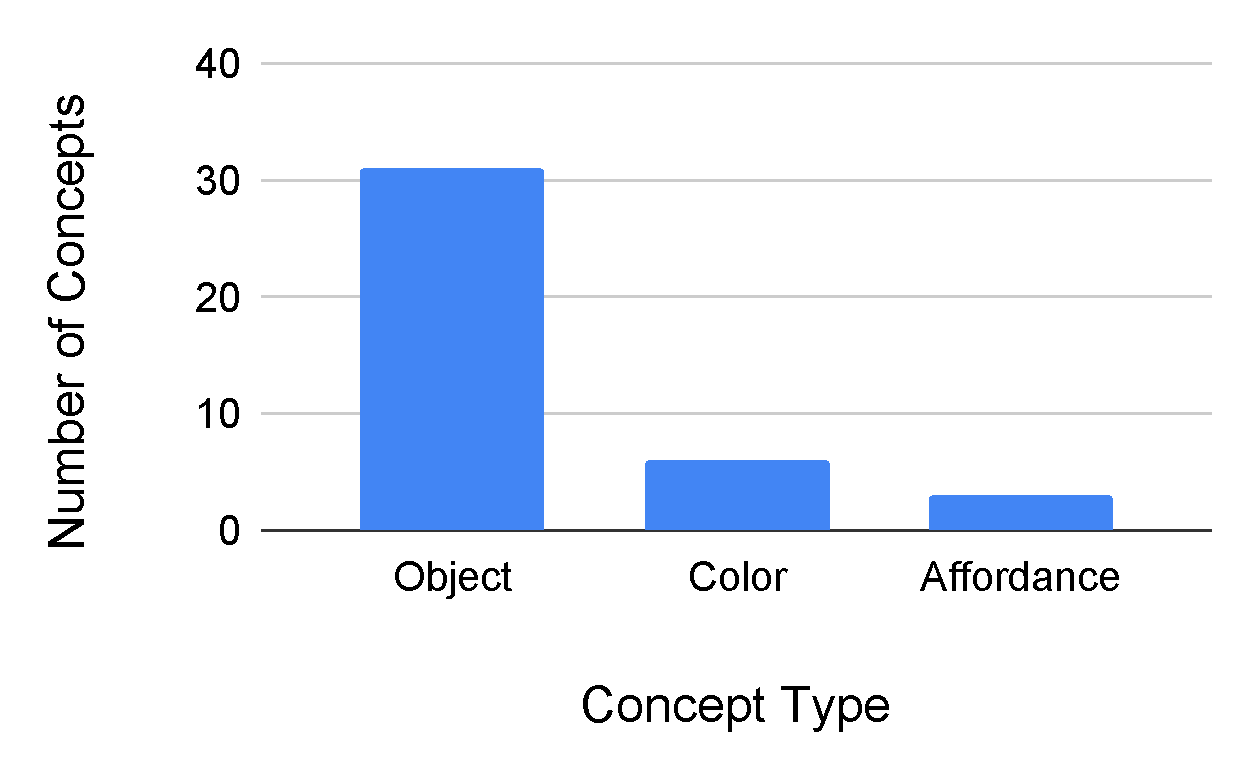
\includegraphics[width=\textwidth]{figures/chart_House.pdf}
  \subcaption{House Construction Domain}
\end{subfigure}
\hspace{0.01\textwidth}
%
\begin{subfigure}{0.28\textwidth}
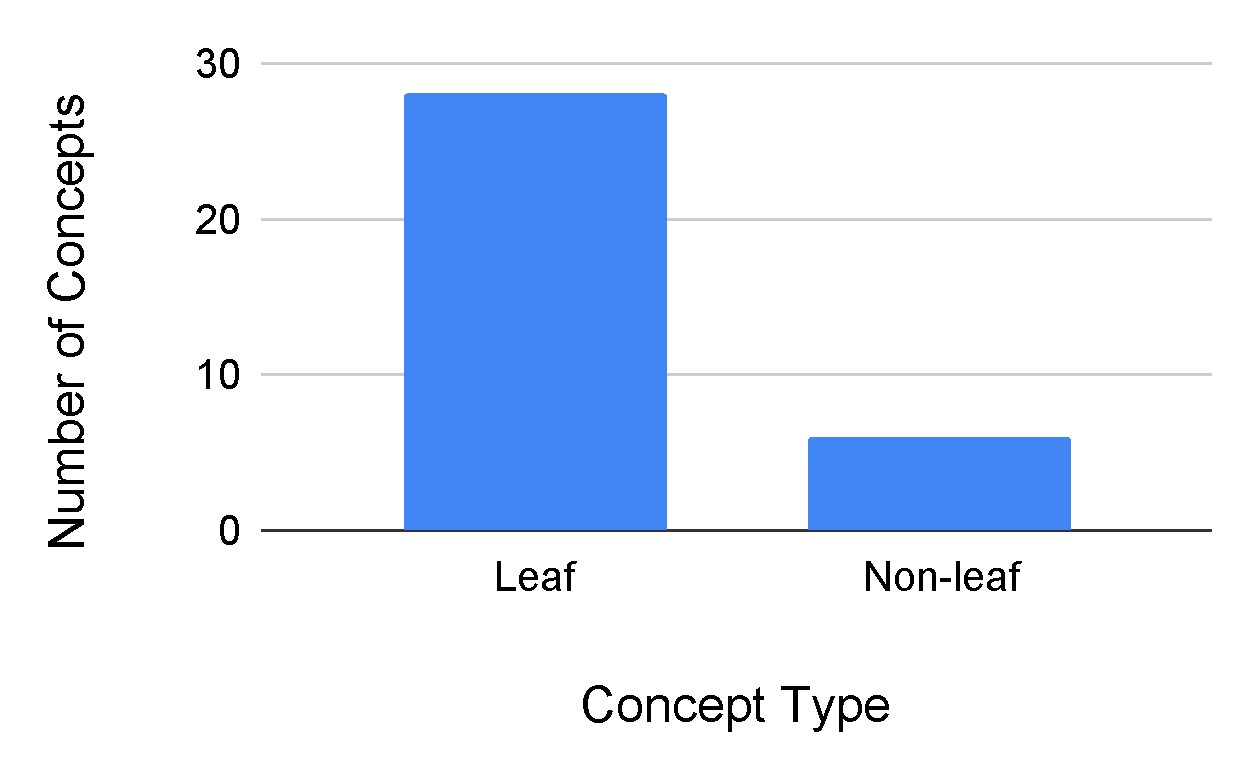
\includegraphics[width=\textwidth]{figures/chart_Zoo.pdf}
  \subcaption{Zoo Domain}
\end{subfigure}


\caption{The number of concepts of each type for all the three domains.}
\label{fig:concept_type}
\end{figure*}

\begin{table*}[t]
\resizebox{\textwidth}{!}{%
\begin{tabular}{c|ccc|ccc}
\toprule
    & Train Image & Test Image & Total Image& Train Concept & Test Concept & Total Concept\\
\midrule
CUB-200-2011 & $8232$ & $3556$ & $11788$ & $307.8$ & $58.2$ & $365$  \\
%\midrule
House& $217$ & $93$ & $310$& $34$ & $6$ & $40$\\
%\midrule
Zoo& $196$ & $84$ & $280$& $28$ & $6$ & $34$\\
\bottomrule
\end{tabular}%
}
\caption{Statistics for the three domains. The number of train and test concepts of the CUB-200-2011 dataset comes from the average of five different splits, resulted in decimal numbers.}
\label{tab:all_stats}
\end{table*}

We split our dataset at two different levels:- the level of concepts and the level of images. The images are divided into $70\%$ for training and $30\%$ for testing, and the testing images are used to evaluate for both seen and unseen concepts. At the concept level, we use five-fold validation. We train the model with $80\%$ of concepts and test on $20\%$ while covering all folds. Because the split of the non-leaf concepts need to guarantee that leaf concepts are unseen as well, our pick of the folds depends on the structure of the concept graph and is not as random as the regular five-fold validation.
The detailed descriptions of each domain are as follows:

\noindent\textbf{CUB-200-2011 dataset}\cite{WahCUB_200_2011} is a standard dataset to demonstrate visual concept learning.
It contains $11,788$ images for $200$ bird classes. Using the following  bird taxonomy\cite{Sullivan2009eBirdAC}, we added the hypernyms of the bird classes and used the bird taxonomy as the hierarchy of concepts.
Following the design of the dense graph propagation~\cite{kampffmeyer2019rethinking}, the relation of each concept includes all of its ancestors.
%Details of the concept relations will be provided in the supplementary materials.

\noindent\textbf{The house construction domain} includes $31$ types of building block objects.
Each object has $10$ different images. 
To introduce relations between concepts, we additionally add $6$ different concepts and $3$ different affordances of objects.
The dataset on the house construction domain includes $310$ images and $40$ concepts in total.
This domain is also used to train the models for the human subject study.
% fillout x from the dataset concepts


\noindent\textbf{The zoo domain} includes $28$ different types of objects. 
Similar to the house domain, we add $6$ general concepts to introduce a hierarchy for the concepts.
The dataset on the zoo domain includes $280$ images and $34$ concepts in total.

Additionally, the detailed statistics of image and concept of each split of each domain are presented in Table~\ref{tab:all_stats}, and the statistics of concept type are presented in Fig.~\ref{fig:concept_type}. Fig.~\ref{fig:sampled_figures} exhibits some sample images from the three domains.
